\documentclass[oneside,hidelinks]{book}
\usepackage{anysize}
\usepackage{amsmath}
\usepackage{mathabx} 
\usepackage{hyperref}
\usepackage{graphicx}
\usepackage{xcolor}
\usepackage[font=small,skip=3pt]{caption}
\usepackage{lmodern}
\usepackage{pdfpages}
\begin{document}
        \tableofcontents
        \parindent=0pt
        \parskip=3pt
        \chapter{Pulse Wave}
                A pulse wave or pulse train is a kind of non-sinusoidal waveform that includes square waves (duty cycle of 50\%)
                 and similarly periodic but asymmetrical waves (duty cycles other than 50\%).
                It is a term used in synthesizer programming, and is a typical waveform available on many synthesizers. 
                The exact shape of the wave is determined by the duty cycle or pulse width of the oscillator output. In many synthesizers, the duty cycle can be modulated (pulse-width modulation) for a more dynamic timbre.[1] The pulse wave is also known as the rectangular wave, the periodic version of the rectangular function.
                       \section{Fortran Code}
                        %kar diyo 
 
                        \subsection{Analytical}
                        \subsection{Numrerical}
                        %likh diy            
                        \section{GNU Script}
                        Analytical:
                        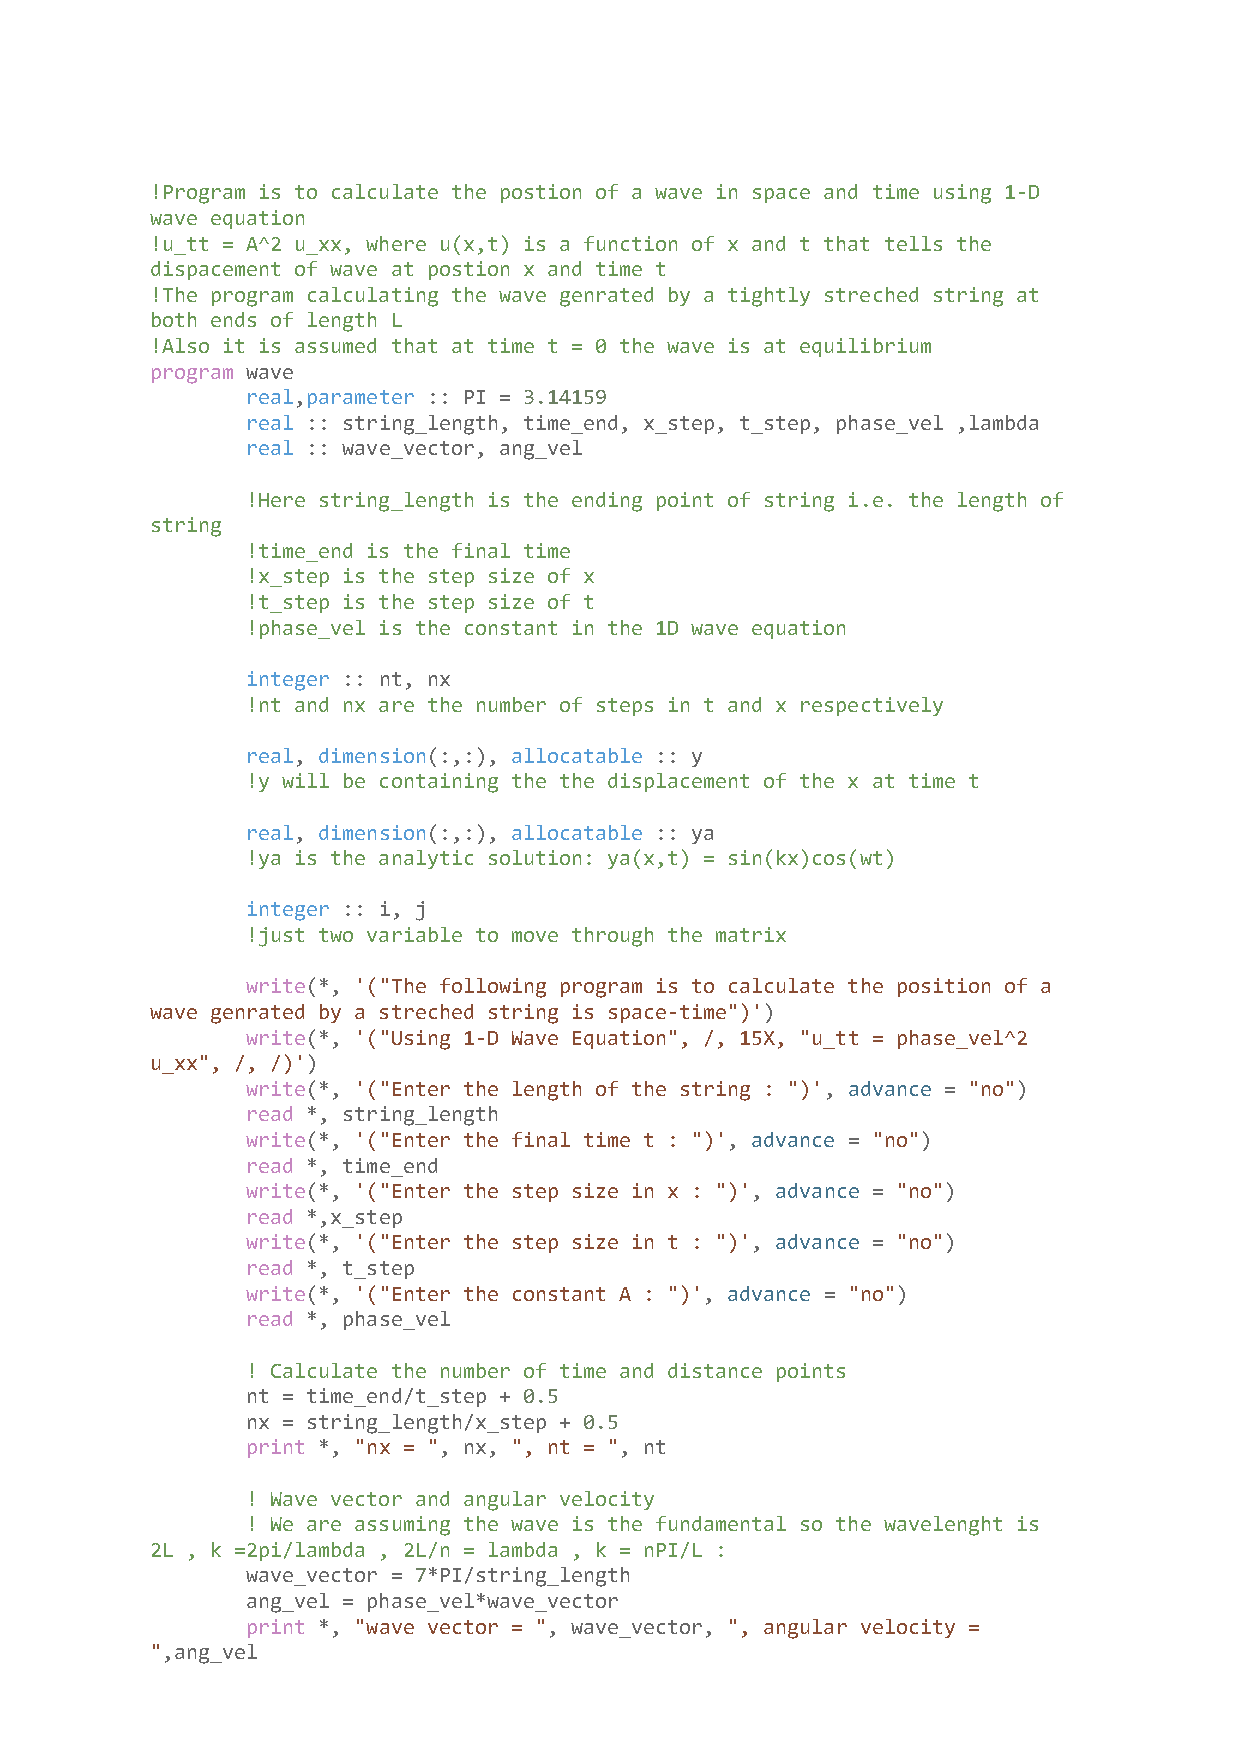
\includepdf[pages={1,2}]{wave.pdf}

                  
\end{document}